\documentclass[12pt]{article}
\usepackage[top=0.85in, bottom=0.5in, left=0.75in, right=0.9in]{geometry}

\usepackage{graphicx,color,enumitem}
\usepackage{amsmath,amsthm,amsbsy}
\usepackage{palatino}

%% Setup aproblem environment, 
%% aproblem items
%% subproblems environment
%% subproblem items
\makeatletter
\newcounter{probcount}
\newcounter{subprobcount}
\newlength\probsep
\newlength\pshrinking
\newif\iffirstprob
\newenvironment{aproblems}%
  {\ifhmode\unskip\par\fi\setcounter{probcount}{0}\probsep\parskip
  \sbox\@tempboxa{\textbf{9.}}\pshrinking\wd\@tempboxa\advance\pshrinking\labelsep
  \let\hproblem\aproblem
  \advance\linewidth -\pshrinking
  \advance\@totalleftmargin\pshrinking
  \advance\leftskip\pshrinking}%
  {\ifhmode\unskip \par\fi\advance\leftskip-\pshrinking}%

\newcommand{\aproblem}{%
  \setcounter{subprobcount}{0}%
  \stepcounter{probcount}%
  \def\@currentlabel{\arabic{probcount}}%
  \ifhmode
    \unskip \par
  \fi
%  \addpenalty{-4000}%
  \iffirstprob\else\addvspace\probsep\fi
  \firstprobfalse
  \hskip -\labelwidth\hskip -\labelsep 
  \hbox to\labelwidth{\hss\textbf{\arabic{probcount}.}}\hskip\labelsep
}%

\newcommand{\subprob}{\item\def\@currentlabel{\arabic{probcount}\alph{\thelistlabel}}}
\newcommand{\skipproblem}{\stepcounter{probcount}}


%% The following commands put defined left and right headers on the top, and a page number
%% on the bottom of all pages beyond page 1
\usepackage{fancyhdr}
\pagestyle{fancy}
\fancyfoot[C]{\ifnum \value{page} > 1\relax\thepage\fi}
\fancyhead[L]{\ifx\@doclabel\@empty\else\@doclabel\fi}
\fancyhead[R]{\ifx\@docdate\@empty\else\@docdate\fi}
\headheight 15pt
\def\doclabel#1{\gdef\@doclabel{#1}}
\def\docdate#1{\gdef\@docdate{#1}}
\makeatother

%% General formatting parameters
\parindent 0pt
\parskip 6pt plus 1pt


\doclabel{Math F251: Section 3.5 Worksheet}
\docdate{Thursday 27 February 2020}


\begin{document}
\renewcommand{\d}{\displaystyle}

\begin{aproblems}
% 3.5 #11
\aproblem  Find $dy/dx$ by implicit differentiation.
    $$y \cos x = x^2 + y^2 \hspace{4.0in}$$
\vfill

% 3.5 #3
\aproblem  Consider the equation
\begin{equation}
\sqrt{x} + \sqrt{y} = 1 \tag{$\ast$}
\end{equation}
\renewcommand{\labelenumi}{(\alph{enumi})}
\begin{enumerate}
\item \quad Find $y'$ by implicit differentiation.
\vfill

\item \quad Solve ($\ast$) explicitly for $y$ and differentiate to get $y'$ in terms of $x$.

\vfill
\item \quad Check that your solutions in (a) and (b) are consistent.

\vfill
\end{enumerate}


\clearpage \newpage
\thispagestyle{empty}
% 3.4 #76
\aproblem  (\emph{A \S3.4 question.})  For what values of $r$ does the function $y= e^{rt}$ satisfy the differential equation $y'' - 4 y' + y = 0$?
\vspace{1.5in}

% 3.5 #29
\aproblem  For the ``cardiod'' shown, with the equation and point given, find an equation of the tangent line.
    $$x^2 + y^2 = (2x^2+2y^2-x)^2, \qquad (0,\tfrac{1}{2}) \hspace{4.0in}$$

\vspace{-0.5in}
\hfill 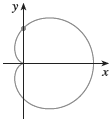
\includegraphics[width=0.25\textwidth]{../../M251S19_F02/worksheets/figs/3p5-29}
\vfill

% 3.5 #39
\aproblem  If $xy+e^y = e$, find the value of $y''$ at the point where $x=0$.
\vfill

\end{aproblems}

\end{document}
